\subsection{Low Rank Structure of Auto-correlation Matrix \texorpdfstring{$\E[\vx\vx^\T]$}{ExxT}}
\label{sec:appendix_xxT}

We have briefly discussed about the autocorrelation matrix $\E[\vx\vx^\T]$ being approximately rank 1 in \sectionref{sec:xxT} in the main text. In particular, we claimed that the mean of layer input dominate the covariance, that $\E[\vx\vx^\T]\approx \E[\vx]\E[\vx^\T]$. In this section we provide some additional empirical results supporting that claim.

We use two metrics to quantify the quality of this approximation: the squared dot product between normalized $\E[\vx]$ and the first eigenvector of $\E[\vx\vx^\T]$ and the ratio between the first and second eigenvalue of $\E[\vx\vx^\T]$. Intuitively if the first quantity is close to 1 and the second quantity is large, then the approximation is accurate.
Formally, for fully connected layers, define $\hE[\vx]$ as the normalized expectation of the layer input $\vx$, namely ${\E[\vx]}/{\|\E[\vx]\|}$.
For convolutional layers, following the notations in \sectionref{sec:appendix_conv}, define $\hE[\vx]$ as the first left singular vector of $\E[\mX]$ where $\hE[\vx]\in \R^{nK_1K_2}$. Abusing notations for simplicity, we use $\E[\vx\vx^\T]$ to denote the $nK_1K_2\times nK_1K_2$ matrix $\E[\mX\mX^\T]$. In this section we consider the squared dot product between $\hE[\vx]$ and the first eigenvector $\vv_1$ of $\E[\vx\vx^\T]$, namely $(\vv_1^\T\hE[\vx])^2$.

For the spectral ratio, let $\lambda_1$ be the first eigenvalue of $\E[\vx\vx^\T]$ and $\lambda_2$ be the second. We have
\begin{equation}
    \frac{\lambda_1}{\lambda_2} \geq \frac{\|\E[\vx]\E[\vx]^\T\|-\|\mSigma_\vx\| }{\|\mSigma_\vx\|} = \frac{\|\E[\vx]\E[\vx]^\T\|}{\|\mSigma_\vx\|} -1,
\end{equation}
where $\mSigma_\vx$ is the covariance of $\vx$. Thus, the spectral norm of $\E[\vx]\E[\vx]^\T$ divided by that of $\mSigma_\vx$ gives a lower bound to ${\lambda_1}/{\lambda_2}$. In our experiments, we usually have
${\lambda_1}/{\lambda_2} \geq {\|\E[\vx]\E[\vx]^\T\|}/{\|\mSigma_\vx\|}$.

As we can see from \tableref{tab:appendix_xxT_spec_fc} and \tableref{tab:appendix_xxT_spec_conv}, in a variety of settings, $\E[\vx]\E[\vx]^\T$ indeed dominated the autocorrelation matrix $\E[\vx\vx^\T]$ for fully connected layers. Similar phenomenon also holds for convolutional layers in the modern architectures, but the spectral gap are generally smaller compared to that of the fully connected layers.
% The values for F-$200^2$(MNIST) and LeNet5 (CIFAR10) are average of 5 different models. From \cref{tab:appendix_xxT_spec} and \cref{fig:appedix_xxT_lowrank} we can see that the $\mathbb{E}[\vx\vx^\T]$ matrix is close to rank 1 for all the models (without batch normalization) we experiment on, and the principle component is approximately $\hE[x]$ from \cref{tab:appendix_xxT_inner}.
 
\newpage

\begin{table}[h]
\small
  \centering
  \caption{Squared dot product $(\vv_1^\T\hE[\vx])^2$ and spectral ratio $\lambda_1/\lambda_2$ for fully connected layers in a selection of network structures and datasets. We independently trained 5 runs for each instance and compute the mean, minimum, and maximum of the two quantities over all layers (except the first layer which takes the input with mean-zero) in all runs.}
  \vskip 0.1in
    \begin{center}
    \begin{tabular}{llccccccc}
    \toprule
         &                  &              & \multicolumn{3}{c}{$(\vv_1^\T\hE[\vx])^2$} & \multicolumn{3}{c}{$\lambda_1/\lambda_2$} \\
Dataset  & Network          & \# fc & mean        & min         & max         & mean         & min          & max         \\
         \midrule
MNIST    & F-$200^2$        & 2            & 1.000       & 1.000       & 1.000       & 12.29        & 9.65         & 16.16       \\
         & F-$600^2$        & 2            & 0.999       & 0.999       & 0.999       & 12.00        & 11.42        & 13.00       \\
         & F-$600^4$        & 4            & 1.000       & 0.999       & 1.000       & 17.81        & 7.33         & 28.00       \\
         & F-$600^8$        & 8            & 0.991       & 0.965       & 1.000       & 6.63         & 2.28         & 11.15       \\
\midrule
CIFAR10  & F-$600^2$        & 2            & 0.999       & 0.998       & 1.000       & 9.24         & 4.74         & 13.74       \\
         & F-$1500^3$       & 3            & 0.999       & 0.997       & 1.000       & 13.27        & 6.10         & 18.41       \\
         & LeNet5           & 3            & 0.998       & 0.997       & 0.999       & 7.21         & 5.88         & 9.02        \\
         & LeNet5-(fc1-80)  & 3            & 0.998       & 0.996       & 0.999       & 7.80         & 6.77         & 11.01       \\
         & LeNet5-(fc1-100) & 3            & 0.997       & 0.995       & 0.999       & 7.42         & 6.20         & 9.10        \\
         & LeNet5-(fc1-150) & 3            & 0.998       & 0.992       & 0.999       & 7.35         & 5.34         & 9.62        \\
         & VGG11-W32        & 1            & 0.990       & 0.988       & 0.993       & 6.02         & 5.57         & 6.51        \\
         & VGG11-W64        & 1            & 0.996       & 0.993       & 0.999       & 5.87         & 5.32         & 6.26        \\
         & VGG11-W64        & 1            & 0.995       & 0.993       & 0.996       & 6.24         & 5.97         & 6.70        \\
\midrule
CIFAR100 & VGG11-W48        & 1            & 0.999       & 0.999       & 0.999       & 17.861       & 15.456       & 20.491      \\
         & VGG11-W64        & 1            & 0.999       & 0.999       & 1.000       & 19.185       & 18.358       & 20.410      \\
         & VGG11-W80        & 1            & 0.999       & 0.999       & 1.000       & 19.455       & 18.120       & 21.450      \\
         & ResNet18-W48     & 1            & 1.000       & 1.000       & 1.000       & 28.23        & 27.37        & 29.27       \\
         & ResNet18-W64     & 1            & 1.000       & 1.000       & 1.000       & 27.07        & 25.72        & 29.50       \\
         & ResNet18-W80     & 1            & 1.000       & 1.000       & 1.000       & 28.23        & 25.98        & 30.03      \\\bottomrule
\end{tabular}
\end{center}
  \label{tab:appendix_xxT_spec_fc}%
\end{table}
\newpage
\begin{table}[h]
\small
  \centering
  \caption{Squared dot product $(\vv_1^\T\hE[\vx])^2$ and spectral ratio $\lambda_1/\lambda_2$ for convolutional layers in the selection of network structures and datasets in \tableref{tab:appendix_xxT_spec_fc}.}
  \vskip 0.1in
    \begin{center}
    \begin{tabular}{llccccccc}
\toprule
         &                  &         & \multicolumn{3}{c}{$(\vv_1^\T\hE[\vx])^2$} & \multicolumn{3}{c}{$\lambda_1/\lambda_2$} \\
Dataset  & Network          & \# conv & mean        & min         & max         & mean         & min          & max         \\
\midrule
CIFAR10  & LeNet5           & 1       & 0.999       & 0.998       & 0.999       & 15.87        & 11.15        & 27.20       \\
         & LeNet5-(fc1-80)  & 1       & 0.998       & 0.998       & 0.999       & 12.36        & 9.53         & 13.36       \\
         & LeNet5-(fc1-100) & 1       & 0.999       & 0.999       & 0.999       & 19.49        & 16.69        & 21.92       \\
         & LeNet5-(fc1-150) & 1       & 0.999       & 0.998       & 0.999       & 12.86        & 7.65         & 16.34       \\
         & VGG11-W32        & 7       & 0.995       & 0.991       & 0.999       & 5.31         & 2.39         & 9.09        \\
         & VGG11-W64        & 7       & 0.997       & 0.993       & 1.000       & 5.76         & 2.50         & 9.98        \\
         & VGG11-W64        & 7       & 0.998       & 0.995       & 1.000       & 5.81         & 2.53         & 10.62       \\
\midrule
CIFAR100 & VGG11-W48        & 7       & 0.996       & 0.991       & 0.999       & 5.72         & 2.46         & 9.90        \\
         & VGG11-W64        & 7       & 0.995       & 0.991       & 0.999       & 5.66         & 2.50         & 10.79       \\
         & VGG11-W80        & 7       & 0.994       & 0.988       & 0.998       & 5.18         & 2.50         & 8.45        \\
         & ResNet18-W48     & 19      & 0.981       & 0.917       & 0.998       & 3.79         & 1.89         & 7.56        \\
         & ResNet18-W64     & 19      & 0.985       & 0.910       & 0.998       & 3.96         & 1.81         & 7.53        \\
         & ResNet18-W80     & 19      & 0.987       & 0.954       & 0.997       & 4.16         & 2.11         & 7.04        \\ \bottomrule
\end{tabular}
\vspace{-0.15in}
\end{center}
  \label{tab:appendix_xxT_spec_conv}%
\end{table}

% \begin{figure}[ht]
%     \centering
%     \begin{subfigure}[b]{0.27\textwidth}
%         \centering
%         \captionsetup{justification=centering}
%         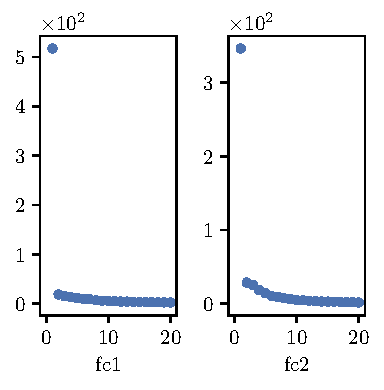
\includegraphics[width=\textwidth]{Figures/Eigenspectrum/xxT/xxT_sigval_d20_MNIST_Exp1_FC2_fixlr0.01R1_E-1_fc1fc2.pdf}

%         \caption{fc1:F-$200^2$ (MNIST)}
%         \label{fig:xxT_sig_lenet_init}%
%     \end{subfigure}
%     \hfill
%     \begin{subfigure}[b]{0.27\textwidth}
%         \centering
%         \captionsetup{justification=centering}
%         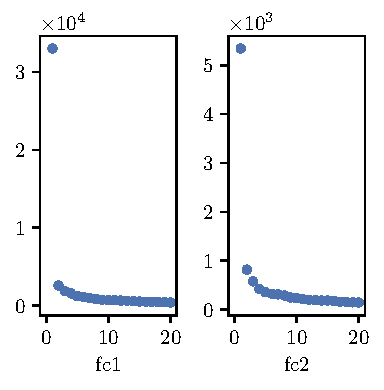
\includegraphics[width=\textwidth]{Figures/Eigenspectrum/xxT/xxT_sigval_d20_CIFAR10_Exp1_LeNet5_fixlr0.01R1_E-1_fc1fc2.pdf}

%         \caption{fc1:LeNet5 (CIFAR10)}
%         \label{fig:xxT_sig_lenet}
%     \end{subfigure}%
%     \hfill
%     \begin{subfigure}[b]{0.27\textwidth}
%         \centering
%         \captionsetup{justification=centering}
%         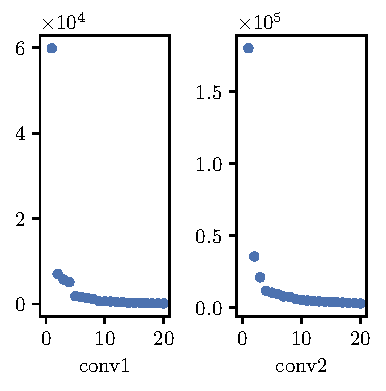
\includegraphics[width=\textwidth]{Figures/Eigenspectrum/xxT/xxTConv_sigval_d20_CIFAR10_Exp1_LeNet5_fixlr0.01_E-1.pdf}

%         \caption{conv1:LeNet5 (CIFAR10)}
%         \label{fig:xxT_sig_lenet_random}
%     \end{subfigure}
%     \captionsetup{justification=centering}

%     \caption{Eigenspectrum of $\E[\vx\vx^\T]$ for different layers in different models. All are close to rank 1.}
%     \label{fig:appedix_xxT_lowrank}
% \end{figure}
\newpage